%\documentclass{exam} 
\documentclass[answers]{exam} 
\usepackage{amsmath,amssymb,enumitem,
fdsymbol,
float,tikz,pgfplots,etoolbox,ifthen,xcolor,fullpage,graphicx,comment,hyperref,environ,array} 
%\usepackage{fontawesome}

\pgfplotsset{compat=1.17}


\usepackage[normalem]{ulem}
\addpoints
\marksnotpoints

\definecolor{MyGreen}{rgb}{0.1, 0.4, 0.1}
\definecolor{MyBlue}{rgb}{0.1, 0.1, 0.9}

\AtBeginEnvironment{solution}{\color{MyGreen}}

\newboolean{NoSolutions} \setboolean{NoSolutions}{true}

%\printanswers (or \noprintanswers) to see the solutions (or not). \noprintanswers is the default so just comment/uncomment the next line. The \setboolean command allows you to use ifthen

\printanswers  \setboolean{NoSolutions}{false}
%\noprintanswers
%Add rubrics
\usepackage{tagging}
% Comment out this line to hide the rubric text:
\usetag{rubric}

\newcommand\pts[1][2]{\textcolor{MyBlue}{\text{\bf [#1 pts]}}}
\newcommand\pt{\textcolor{MyBlue}{\text{\bf [1 pt]}}}

\newcommand\rubric[1]{\tagged{rubric}{\textcolor{MyBlue}{#1}}}

\newenvironment{rubricEnv}{\taggedblock{rubric} \color{MyBlue}}{\endtaggedblock}

\newcommand{\onestar}{\raisebox{0.05cm}{\resizebox{1.6cm}{!}{$\bigstar\largewhitestar\largewhitestar\largewhitestar$ \ }}}
\newcommand{\twostar}{\raisebox{0.05cm}{\resizebox{1.6cm}{!}{$\bigstar\bigstar\largewhitestar\largewhitestar$ \ }}}
\newcommand{\threestar}{\raisebox{0.05cm}{\resizebox{1.6cm}{!}{$\bigstar\bigstar\bigstar\largewhitestar$ \ }}}
\newcommand{\fourstar}{\raisebox{0.05cm}{\resizebox{1.6cm}{!}{$\bigstar\bigstar\bigstar\bigstar$ \ }}}

\newcommand{\lr}[3]{\left#1{\mathstrut#3}\right#2}
\renewcommand{\half}{\frac{\textstyle 1}{\textstyle 2}}
\renewcommand{\o}{\omega}
\renewcommand{\a}{\alpha}
\renewcommand{\b}{\beta}
\renewcommand{\bar}[1]{\mskip.5\thinmuskip\overline{\mskip-.5\thinmuskip {#1} \mskip-.5\thinmuskip}\mskip.5\thinmuskip}


\everymath{\displaystyle}
\newcommand{\diff}[2]{\frac{\text{d}#1}{\text{d}#2}}


\begin{document}

\subsection*{MATH 101A --- ASSIGNMENT 1}

\subsubsection*{Learning goals}
\begin{itemize}
    \setlength\itemsep{0.1em}
    \item Compute the average value of a given function on a given interval.
    \item Calculate moving averages for a given time-varying function.
    \item Interpret integrals involving flow rates in practical terms.
    \item Confront the Keeling curve and its consequences.
\end{itemize}

\subsubsection*{Contributors}

\textit{On the first page of your submission, list the student numbers and full names (with the last name in \textbf{bold}) of all team members. Indicate members who have not contributed using the comment ``(non-contributing)''.}

\begin{itemize}
    \item \#00000000 Randy {\bf Zhu}
\end{itemize}

\subsubsection*{Reflection question}

\textit{Reflection questions encourage you to think about how mathematics is done. This is an important ingredient of success. Reflection questions contribute to your \textbf{engagement grade}.}

\begin{questions}

\question To work productively as a team, it is helpful to have shared expectations. This question consists of prompts that form a ``team contract'', a document that guides how you will work together. Before answering the prompts, read the document ``Group resources'' that is posted along with the assignment on the Canvas course page.

\begin{parts}
    \part What are your overarching ``ground rules''? Come up with 4-6 specific expectations regarding communication (including how often and what medium), meetings (how often, how long, and where), preparation and attendance.
    \part What actions will your team take if a member does not follow the ground rules? Be specific.
    \part What happens if a team member does not fulfill an agreed-upon task for an assignment? Consider both how the team will handle any dropped tasks, as well as  actions you will take as a team.

\end{parts}

\end{questions}

\begin{solution}
    Put your answers here.
    \begin{parts}
    
    \part
    
    \begin{itemize}
        \item We will embrace collaboration, an acceptance of each others' ideas with an open mind and respect.
        \item Participate in group work to the best of our ability.
        \item We'll communicate the issues to that we run into, and try to help eachother with said blockers.
        \item We'll meet well before the assignment deadline, again, to the best of our ability.
    \end{itemize}
    
    \part
    
    We will have a group conversation to find out the root cause of the issue, and rectify it. If this is not handled, we will report them to the TAs/teaching team of the course.

    \part Answer to 1(c) goes here.

    We will support our group member in doing the task and we'll like them catch up, or
    re-assign the task to another member.
    
\end{parts}
\end{solution}



\vfill\clearpage

\subsubsection*{Assignment questions}

\noindent
\textit{The questions in this section contribute to your \textbf{assignment grade}.
Stars indicate the difficulty of the questions, as described on Canvas.}

\noindent
\textit{Parts (\ref{sineaverage}), (\ref{quadratic}), and (\ref{cosinelags}) of Question~2
require plots. We will accept either careful handmade sketches or 
computer-generated graphics, as produced by software like Desmos.}

\bigskip

\noindent
The graph below may be the most important one you study all year.
It shows the concentration of CO$_2$ in the atmosphere as a function of time,
which has a strong influence on the global climate.
\[
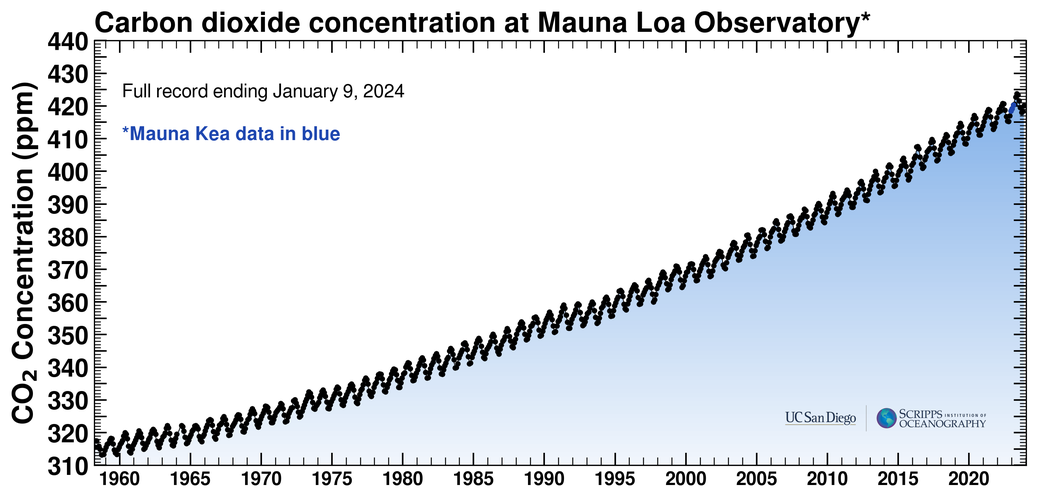
\includegraphics[scale=0.35]{maunaloa2.png}
\]
\[\text{\textbf{Fig.~1:} CO$_2$ concentrations in recent years}\]
Today's CO$_2$ levels have never been seen before in human history,
and they will cause enormous global changes in the next few decades.
Understanding this graph in detail will be an important step
in preparing for, perhaps even influencing,
the immediate future of humanity and indeed all life on Earth.

\begin{questions}\setcounter{question}{1} 

\question[12]
There is a clear increasing trend in Figure~1,
but there are also short-term ripples.
To systematically remove the ripples
and extract the trend,
we can use a \emph{moving average}.

For any integrable function $f$ and interval $[a,b]$,
the \emph{average value of $f$ on $[a,b]$} is the number
$f_{\rm AV}$ defined by
\[
f_{\rm AV} = \dfrac{1}{b-a}\int_a^b f(t)\,dt.
\]
Rearranging this definition reveals a natural interpretation:
\[
\int_a^b f(t)\,dt
= (b-a) f_{\rm AV}
= \int_a^b f_{\rm AV}\,dt.
\]
The number $f_{\rm AV}$ is \emph{the unique constant} 
that produces the same integral as $f$ over $[a,b]$.

\begin{parts} \label{sineaverage}
\part\onestar
Calculate the average value of the function $f(t)=\sin(t)$ on the interval $[0,\pi]$.
Then plot the graphs of $y=f(t)$ and $y=f_{\rm AV}$ on the same set of axes,
restricting the sketch to $0\le t\le\pi$.

\begin{solution}

\[ f_{\text{AV}} = \frac{1}{\pi} \int^{\pi}_{0} \sin(t)dt = \frac{1}{\pi} \big(-\cos(t)\Big|^{\pi}_0\big) = \frac{1}{\pi} (-\cos(\pi) - -\cos(0))    = \frac{2}{\pi} \]

\centering
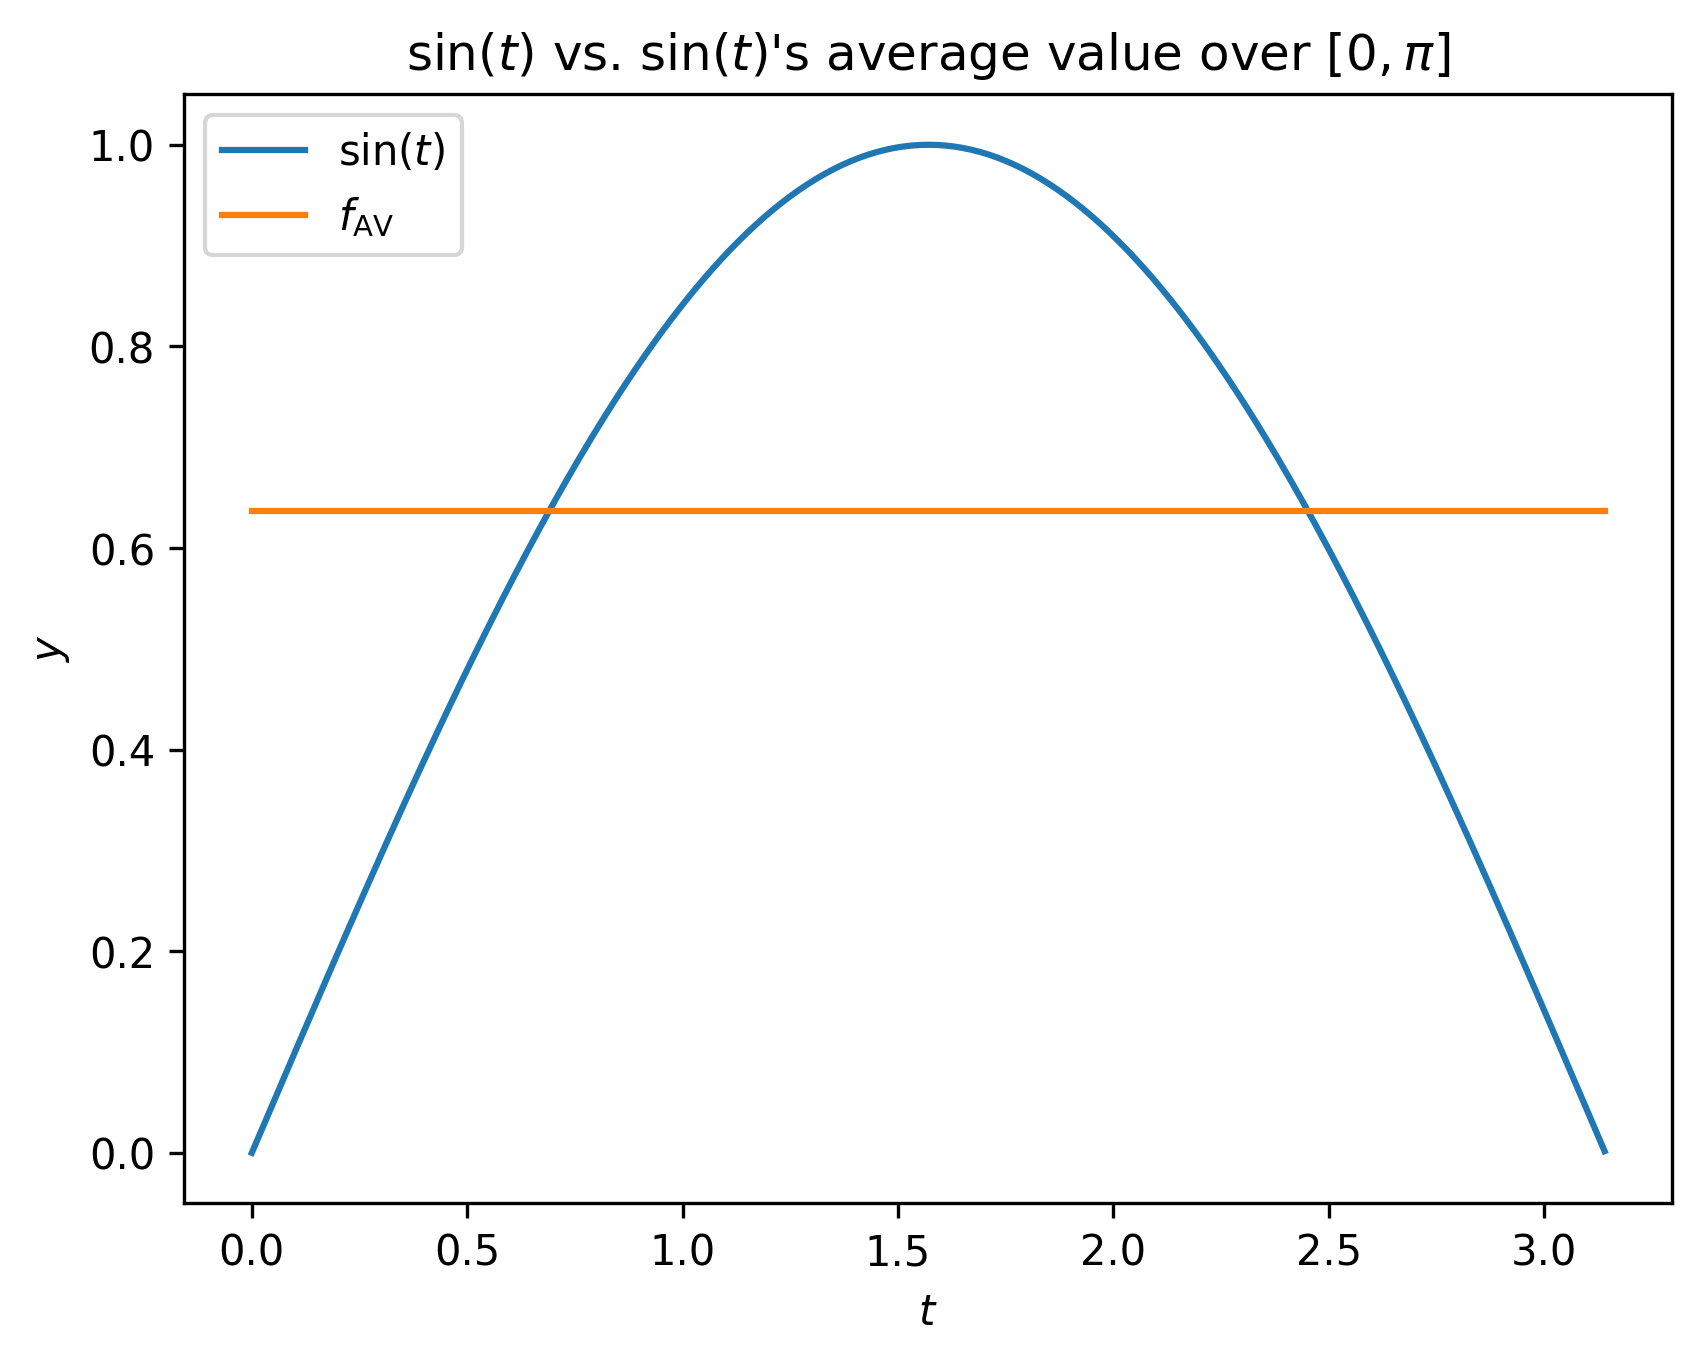
\includegraphics[scale=0.18]{2a_plot.png}

\end{solution}

\part\onestar
Calculate the average value of the function $f(t) = t^2$ on the interval $[1,2]$.
Then plot the graphs of $y=f(t)$ and $y=f_{\rm AV}$ on the same set of axes,
restricting the sketch to $1\le t\le 2$.

\begin{solution}

\[ f_{\text{AV}} = \frac{1}{2 - 1} \int^{2}_{1} t^2 dt = \frac{1}{3}t^3 \Big|^{2}_{1} = \frac{1}{3}(2)^3 - \frac{1}{3}(1)^3 = \frac{7}{3} \]

\centering
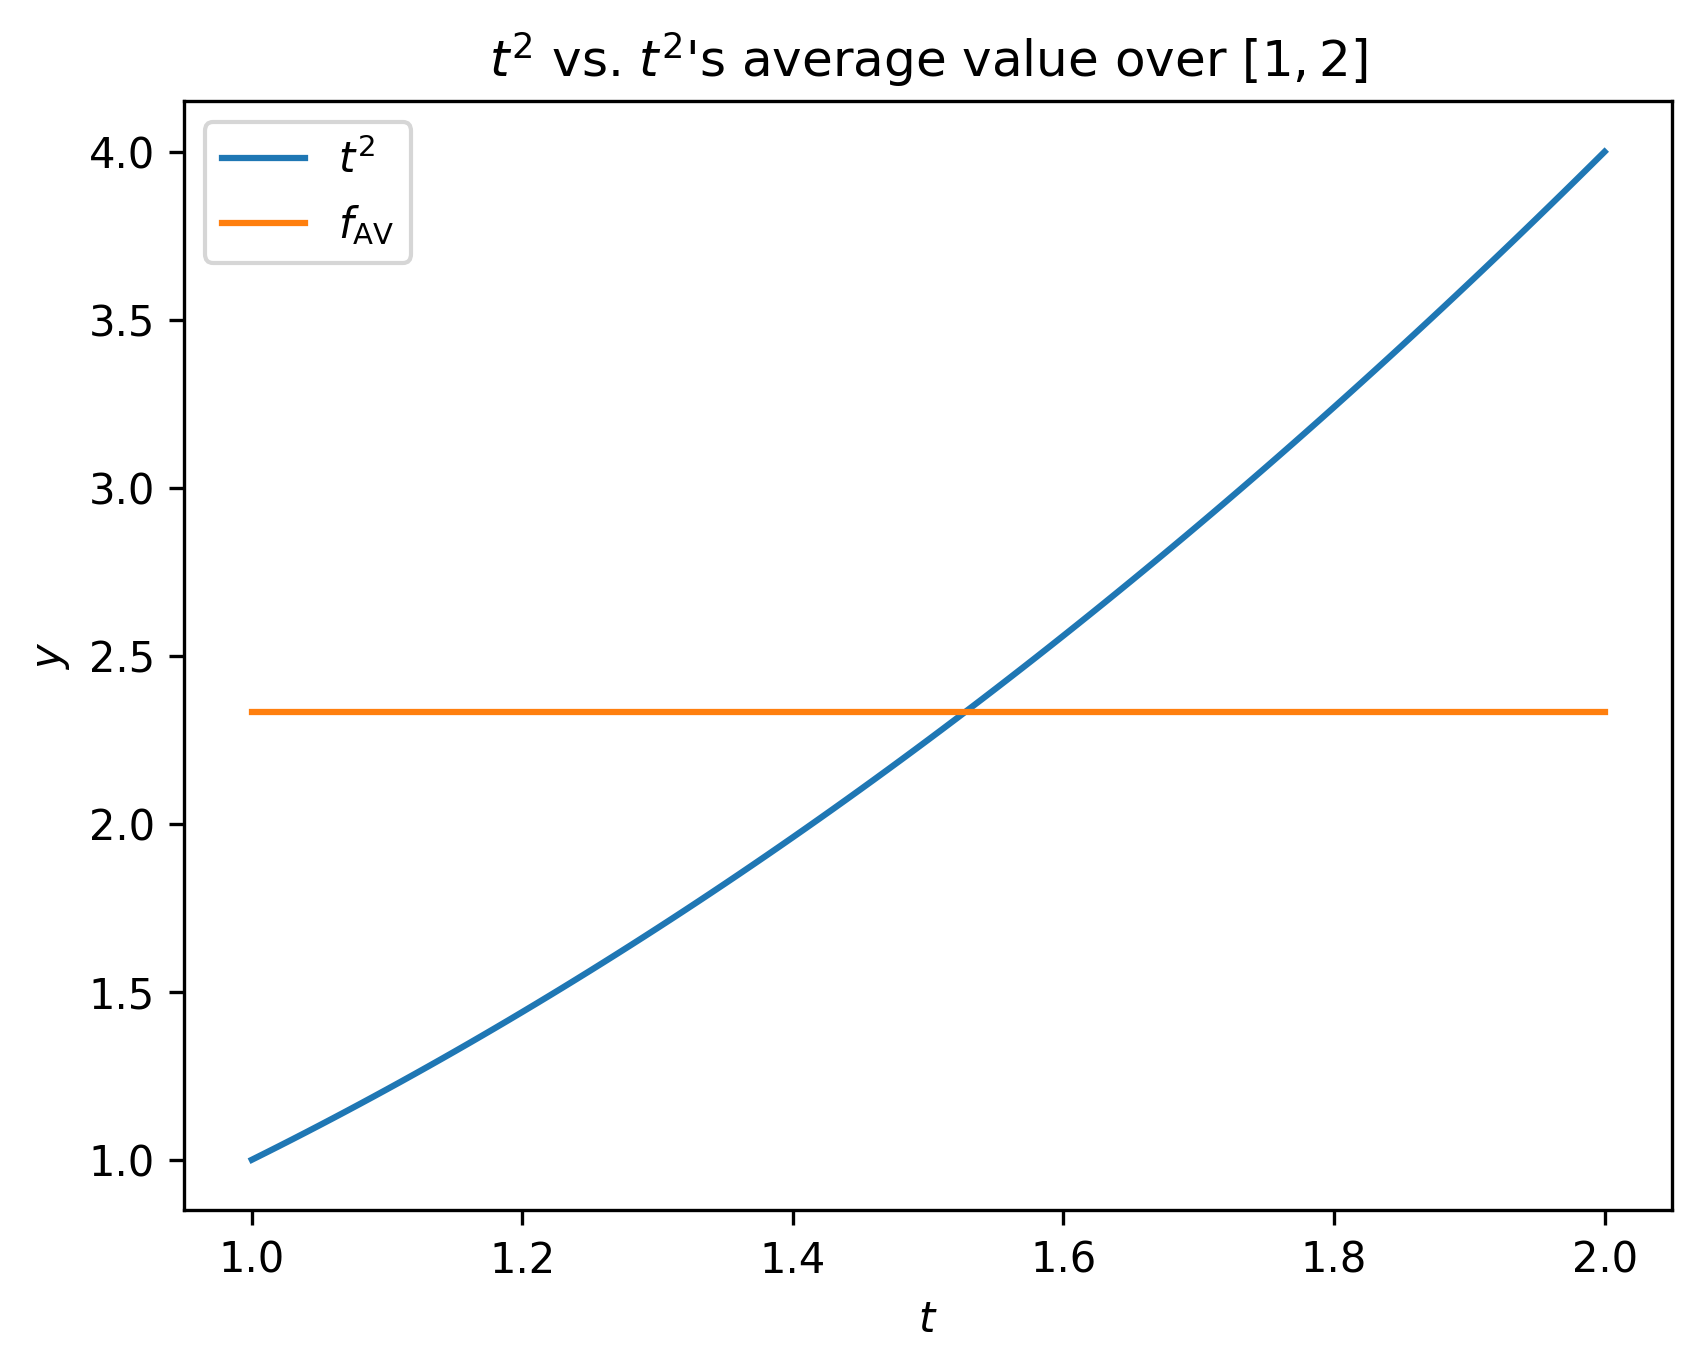
\includegraphics[scale=0.18]{2b_plot.png}

\end{solution}


\begin{EnvUplevel}
Now imagine that some time-varying function $f$ is given.
If we pick some number $r>0$, we can imagine the interval $[t-r,t]$
as a moving window of width $r$ and final time $t$.
Calculating the average value of $f$ over this window
will produce a result that depends on $t$, 
thus defining a new function $\bar f$ as follows:
\[
\bar f(t) = \dfrac{1}{r} \int_{t-r}^{t} f(x)\,dx.
\]
Let's investigate the relationship between $f$ and $\bar f$
in various situations.
\end{EnvUplevel}

\part\onestar \label{powers}
Let $f_0(t)=1$, $f_1(t)=t$, and $f_2(t)=t^2$.
Find $\bar f_0(t)$, $\bar f_1(t)$, and $\bar f_2(t)$.
(The results may depend on $r$.)

\begin{solution}
    Intuitively, the result for $f_0(t) = 1$ makes sense as the average value of something that's constant is always that constant value.
    \[ \bar f_0(t) = r^{-1} \int^{t}_{t - r} 1dx = r^{-1} \Big(x \Big|^{t}_{t - r}\Big) = r^{-1}(t - (t - r)) = 1 \]
        
    \[ \bar f_1(t) = r^{-1} \int^{t}_{t - r} xdx = r^{-1} \Big(\frac{1}{2}x^2\Big|^{t}_{t-r}\Big) = r^{-1}(\frac{1}{2}(t)^2 - \frac{1}{2}(t - r)^2) = t - \frac{1}{2}r \]

    \[ \bar f_2(t) = r^{-1} \int^{t}_{t - r} x^2dx = r^{-1} \Big(\frac{1}{3}x^3\Big|^{t}_{t-r}\Big) = r^{-1}(\frac{1}{3}t^3 - \frac{1}{3}(t - r)^3) = t^2 - rt + \frac{1}{3}r^2 \]

    The fractional term seems to cancel out, and so when $r=0$ or $r \to 0$, we get our function back, I wonder where we've seen that...
\end{solution}

\part\onestar \label{quadratic}
Express $\bar f(t)$ in terms of $r$ for the general quadratic
$f(t) = at^2 + bt + c$, where $a,b,c$ are real constants.

\begin{solution}
    Exploiting the results from (c), and the linearity of integrals,

    \begin{align*}
        \bar f(t) &= r^{-1} \int^{t}_{t - r} ax^2 + bx + c dx = a r^{-1}\int^{t}_{t-r} x^2 dx + b r^{-1}\int^{t}_{t-r} xdx + c r^{-1}\int^{t}_{t-r} 1dx \\
                  &= a\big( t^2  - rt + \frac{1}{3} r^2 \big) + b\big( t - \frac{1}{2}r \big) + c \\
                  &= \frac{1}{3}ar^3 + at^2 - art + bt - \frac{1}{2}br + c
    \end{align*}

    saves us from a lot of algebra.
    
\end{solution}

\part\onestar \label{cosine}
Given a constant $\o>0$, let $g(t) = \cos(\o t)$.
Find $\bar g(t)$ in terms of $r$ (and, of course, $\o$).

\begin{solution}
    Left in a convenient format for the next question
    \begin{align*}
        \bar g(t) &= r^{-1} \int^{t}_{t - r} \cos(\o x) dx = r^{-1} \Big( \frac{1}{\o}\sin(\o x) \Big|^{t}_{t-r} \Big) = \frac{1}{\o}\sin(\o t) - \frac{1}{\o}\sin(\o(t - r)) \\
                  &= \frac{\frac{1}{\o}\sin(\o t) - \frac{1}{\o} \sin(\o (t - r))}{r}
    \end{align*}
\end{solution}

\part\threestar \label{shortwindoweg}
It's reasonable to expect that a moving average with a very short window
should produce a new function very close to the original one,
provided the original function is continuous.
Test this expectation on the functions from parts~(\ref{quadratic}) and~(\ref{cosine}) above
by taking the limit as $r\to 0^+$ in your expressions
for $\bar f(t)$ and $\bar g(t)$.

\begin{solution}
    \[ \lim_{r \to 0^+} \bar f(t) = \lim_{r \to 0^+} \frac{1}{3}ar^3 + at^2 - art + bt - \frac{1}{2}br + c \]
    As $\bar f(t)$ is continuous everywhere, we can ``plug in" $0$ for $r$, and this yields
    \[  \lim_{r \to 0^+} \bar f(t) = at^2 + bt + c \]

    $\bar g(t)$ is a little more complicated,
    \[ \lim_{r \to 0^+} \bar g(t) = \lim_{r \to 0} \frac{\frac{1}{\o}\sin(\o t) - \frac{1}{\o} \sin(\o (t - r))}{r} \]

    As $\lim_{r \to 0^+} \frac{1}{\o}\sin(\o t) - \frac{1}{\o}\sin(\o ( t- r)) = 0$, $\frac{1}{\o}\sin(\o t) - \frac{1}{\o}\sin(\o ( t- r))$ is differentiable everywhere w.r.t. $r$, $\lim_{r \to 0^+} r = 0$, and $r$ is differentiable everywhere, $\bar g(t)$ is a candidate for L'Hopital's rule.

    By L'Hopital's rule,

    \[\lim_{r \to 0^+} \bar g(t) = \lim_{r \to 0^+} \frac{\frac{d}{dr} [\frac{1}{\o}\sin(\o t) - \frac{1}{\o}\sin(\o ( t- r))]}{\frac{d}{dr} [r]} = \lim_{r \to 0^+} \frac{\cos(\o t - \o r)}{1} = \cos(\o t) \]
\end{solution}


\part\twostar \label{derivative}
For a generic continuous function $h$,
find an algebraic formula involving $r$ for $\bar h'(t)$.


\begin{solution}
    Let $H(x)$ be the antiderivative of $h(x)$ (i.e., let $H(x)$ satisfy the identity $H'(x) = h(x)$).

    By definition,
    
    \[ \bar h(t) = \frac{1}{r} \int^{t}_{t - r} h(x)dx \]

    By FTC2,

    \[  \bar h(t) = \frac{1}{r} (H(t) - H(t - r))\]

    Differentiating yields us,

    \[ \bar h'(t) = \frac{d}{dt} \frac{1}{r} (H(t) - H(t - r)) = \frac{1}{r}(h(t) - h(t - r)) = \frac{h(t) - h(t - r)}{r} \]
\end{solution}


\part\onestar \label{cosinelags}
For this part only, define $g(t)=\cos(2\pi t)$
and use $r=\half$ to define $\bar g(t)$.
Plot both $y=g(t)$ and $y=\bar g(t)$ for $0\le t\le 4$
on the same axes.


\begin{solution}

    \centering
    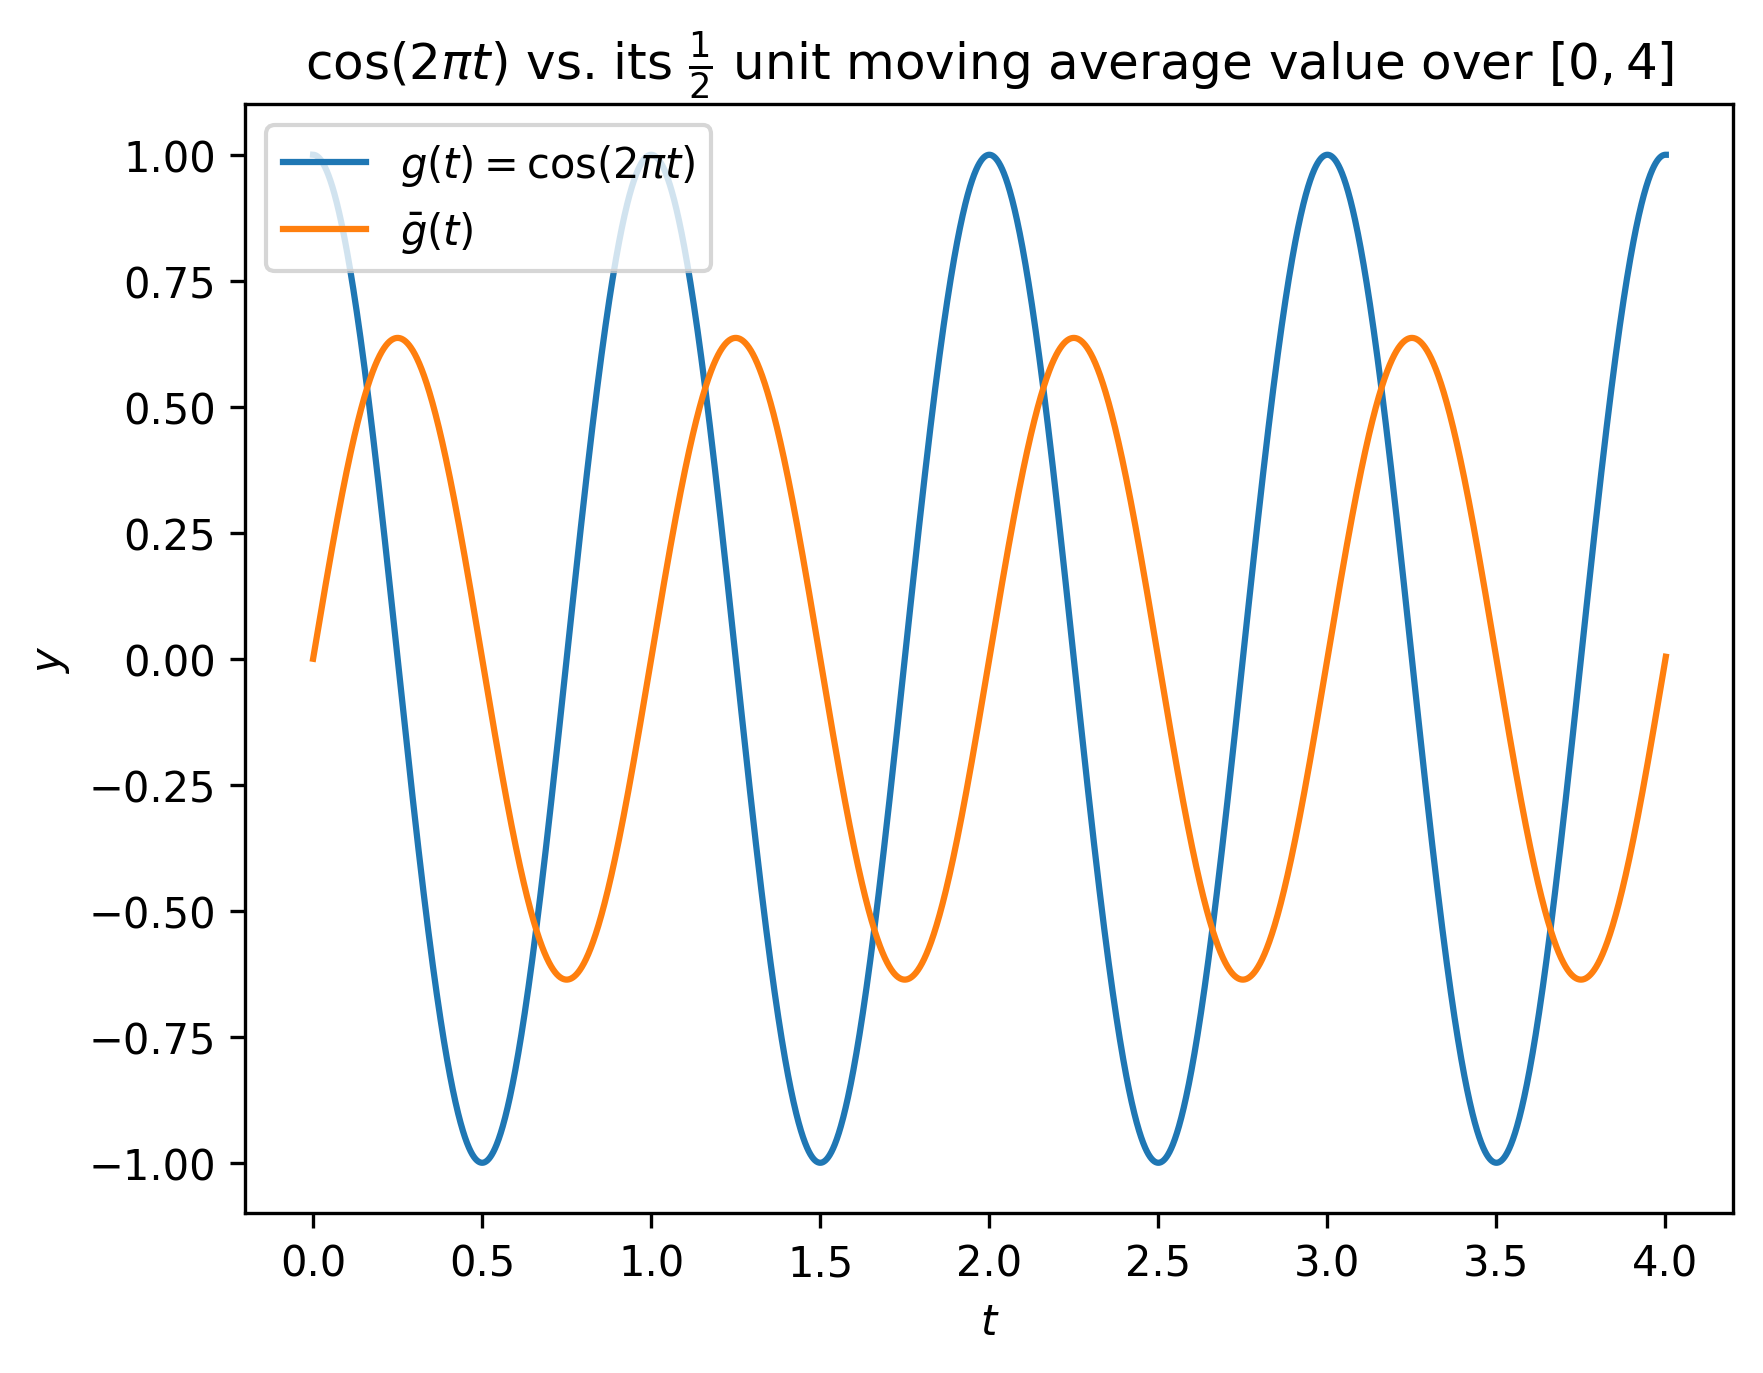
\includegraphics[scale=0.18]{image.png}
    
\end{solution}


\part \twostar Look at the maximum and minimum values on your plot in part~(\ref{cosinelags}).
Notice that
\begin{enumerate}
\item the extreme values of $\bar g(t)$
\emph{occur later} than the extreme values of $g(t)$, 
and
\item the extreme values of $\bar g(t)$
\emph{are smaller in magnitude} than the extreme values of $g(t)$.
\end{enumerate}
Write brief intuitive explanations of these two facts.
(\emph{Note\/}: 
``That's what the calculations produce'' is simultaneously
(i)~logically correct, and (ii)~a dreadful intuitive explanation.)


\begin{solution}

    We're considering the average value between $[t-r, t]$, this means that our function takes a ``snapshot" of the interval, rather than a ``local" look at the function. This means that as we're at a maxima, the function still ``remembers" the values previous to the maxima, which are lower than the maxima. A similar case holds for the minima, where the previous greater values are ``remembered" by the function. This leads to a delayed extreme value in the function.

    In terms of magnitude, because the function ``remembers" the previous values, it cannot be greater than the local maxima, because all local extrema of the function $\cos(2 \pi t)$ are the equal, which means the average must be lesser in magnitude than the extrema.
    
\end{solution}

\part\threestar \label{shortwindow}
Extend your observations in part~(\ref{shortwindoweg}) above to 
explain why taking the limit as $r\to 0^+$ in the definition
of $\bar h(t)$ will recover the original value of $h(t)$,
for any given continuous function $h$.
\\
(\emph{Hint\/}:
This question is \emph{fundamental}.
You have confronted it before.)

\begin{solution}
    By definition, 
    \[ \bar h(t) = \frac{1}{r} \int^{t}_{t - r} h(x)dx \]
    Re-arranging, we have:
    \[ \bar h(t) = \frac{\int^{t}_{t - r} h(x)dx}{r} \]
    Let $H$ be an arbitrary antiderivative of $h$, we apply the Fundamental Theorem of Calculus, part 2,
    \[  \bar h(t) = \frac{H(t) - H(t - r)}{r} \]
    Doing some algebraic manipulation, we get,
    \[ \bar h(t) = \frac{H(t) - H(t - r)}{r} = \frac{-H(t - r) + H(t)}{r} = -\frac{H(t - r) - H(t)}{r} \]
    This looks so close to the definition of the derivative, so we will take the limit as $r \to 0^+$ now,
    \[ \lim_{r \to 0^+} -\frac{H(t - r) - H(t)}{r} \]
    Let use perform a variable interchange and limit direction,
    \[ \lim_{r \to 0^-} -\frac{H(t + r) - H(t)}{-r} = \lim_{r \to 0^-} \frac{H(t + r) - H(t)}{r} = H'(t) \]

    By our definition of $H$, and the Fundamental Theorem of Calculus Part 1
    , we have $H' = h$, as required.
\end{solution}

\part\twostar \label{cosinekiller}
When $g(t)=\cos(\o t)$ as above, 
some special values of $r>0$ are 
extremely effective at removing ripples.
Find all $r>0$ for which $\bar g(t)$ is a constant function.
(Expect the answers to involve $\o$.)


\begin{solution}
    Because $\bar g'(t) \iff \bar g(t)$ is constant, we can find where values of $r$ where $\bar g'(t) = 0$ to find what values of $r$ makes $\bar g(t)$ constant.

    \begin{align*}
        \frac{\cos(\o t) - \cos(\o (t - r)}{r} &= 0 \\
        \cos(\o t) - \cos(\o (t - r)) & = 0 \\
        \o t &= \o t - \o r + 2\pi n \tag{for $n \in \mathbb{Z}^+$, as cosine is periodic} \\
        r &= \frac{2 \pi}{\o}n
    \end{align*}
\end{solution}



\end{parts}

\question[5]
Figure~1 shows that the CO$_2$ concentration 
in the atmosphere varies from season to season.
Photosynthesis helps explain this: 
there is more land, and therefore more plant material,
in Earth's northern hemisphere than in the south.
When the northern hemisphere is having summer,
plants absorb CO$_2$ and turn it into tissue.
When it is winter in the north,
the plants slow down their absorption and the humans 
turn up their emissions.
It's summer in the south,
but there aren't enough plants there to compensate for 
all this and keep the absorption rate steady.

Suppose $M(t)$ denotes the total mass of CO$_2$ in the atmosphere
at time $t$, measuring time $t$ in years from the usual Year~0,
and measuring mass in kg.
Then we can write
\[
\frac{dM}{dt}=i(t)-o(t),
\]
where $i(t)$ is the rate at which CO$_2$ is added to the atmosphere due to respiration and emissions 
[``influx'']
and $o(t)$ is the rate at which CO$_2$ leaves the atmosphere due to photosynthesis and other effects
[``outflux''].

\begin{parts}

\part \onestar Let $t_0 \geq 0$ and $t_1 > t_0$ represent two different points in time. 
Write a brief description, including units, for the physical meaning of the
integrals shown below:
    \begin{itemize}
            \item  $\int_{t_0}^{t_1} i(t)\,dt$,
            \item   $\int_{t_0}^{t_1} \left(i(t) - o(t)\right)\,dt$.
     \end{itemize}
\begin{solution}
    The first integral represents the total mass of CO\textsubscript{2} in kilograms added into the atmosphere from year $t_0$ to $t_1$.

    The second integral represents the net change in total mass (still in kilograms) over year $t_0$ to $t_1$.
\end{solution}

\begin{EnvUplevel}
The total mass of the atmosphere changes slowly enough to be treated as a constant, $M_0$.
Define $C(t) = 10^6\,M(t)/M_0$: 
since both $M(t)$ and $M_0$ are measured in kg,
their ratio is a pure number with no units.
Multiplying that ratio by $10^6$ produces numbers of convenient sizes,
and explains the description of $C(t)$ as a concentration in ``parts per million (ppm)''.
This is the function plotted in Figure~1.
\end{EnvUplevel}


\begin{EnvUplevel}
If the ripples in Figure~1 are really caused by the seasons,
their influence might have a form like $\cos(\o t)$, with $\o$
chosen so that a full cycle takes exactly one year.
This calls for $\o=2\pi$ (with units y$^{-1}$).
With the results of problem~2(\ref{cosinekiller}) above in mind, we choose $r = 2\pi/\o = 1$ (units: y)
and introduce
\[
\bar C(t) = \dfrac{1}{r}\int_{t-r}^t C(x)\,dx = \int_{t-1}^t C(x)\,dx.
\]
The accurate measurements plotted in Fig.~1 are freely available online.
They are tabulated monthly, so anyone can use the Trapezoidal Rule with $12$
subintervals to calculate a good approximation for $\bar C(t)$ at each
measurement time $t$.
The next plot shows the graphs of the measured function $C(t)$
and the computed values of $\bar C(t)$.
\[
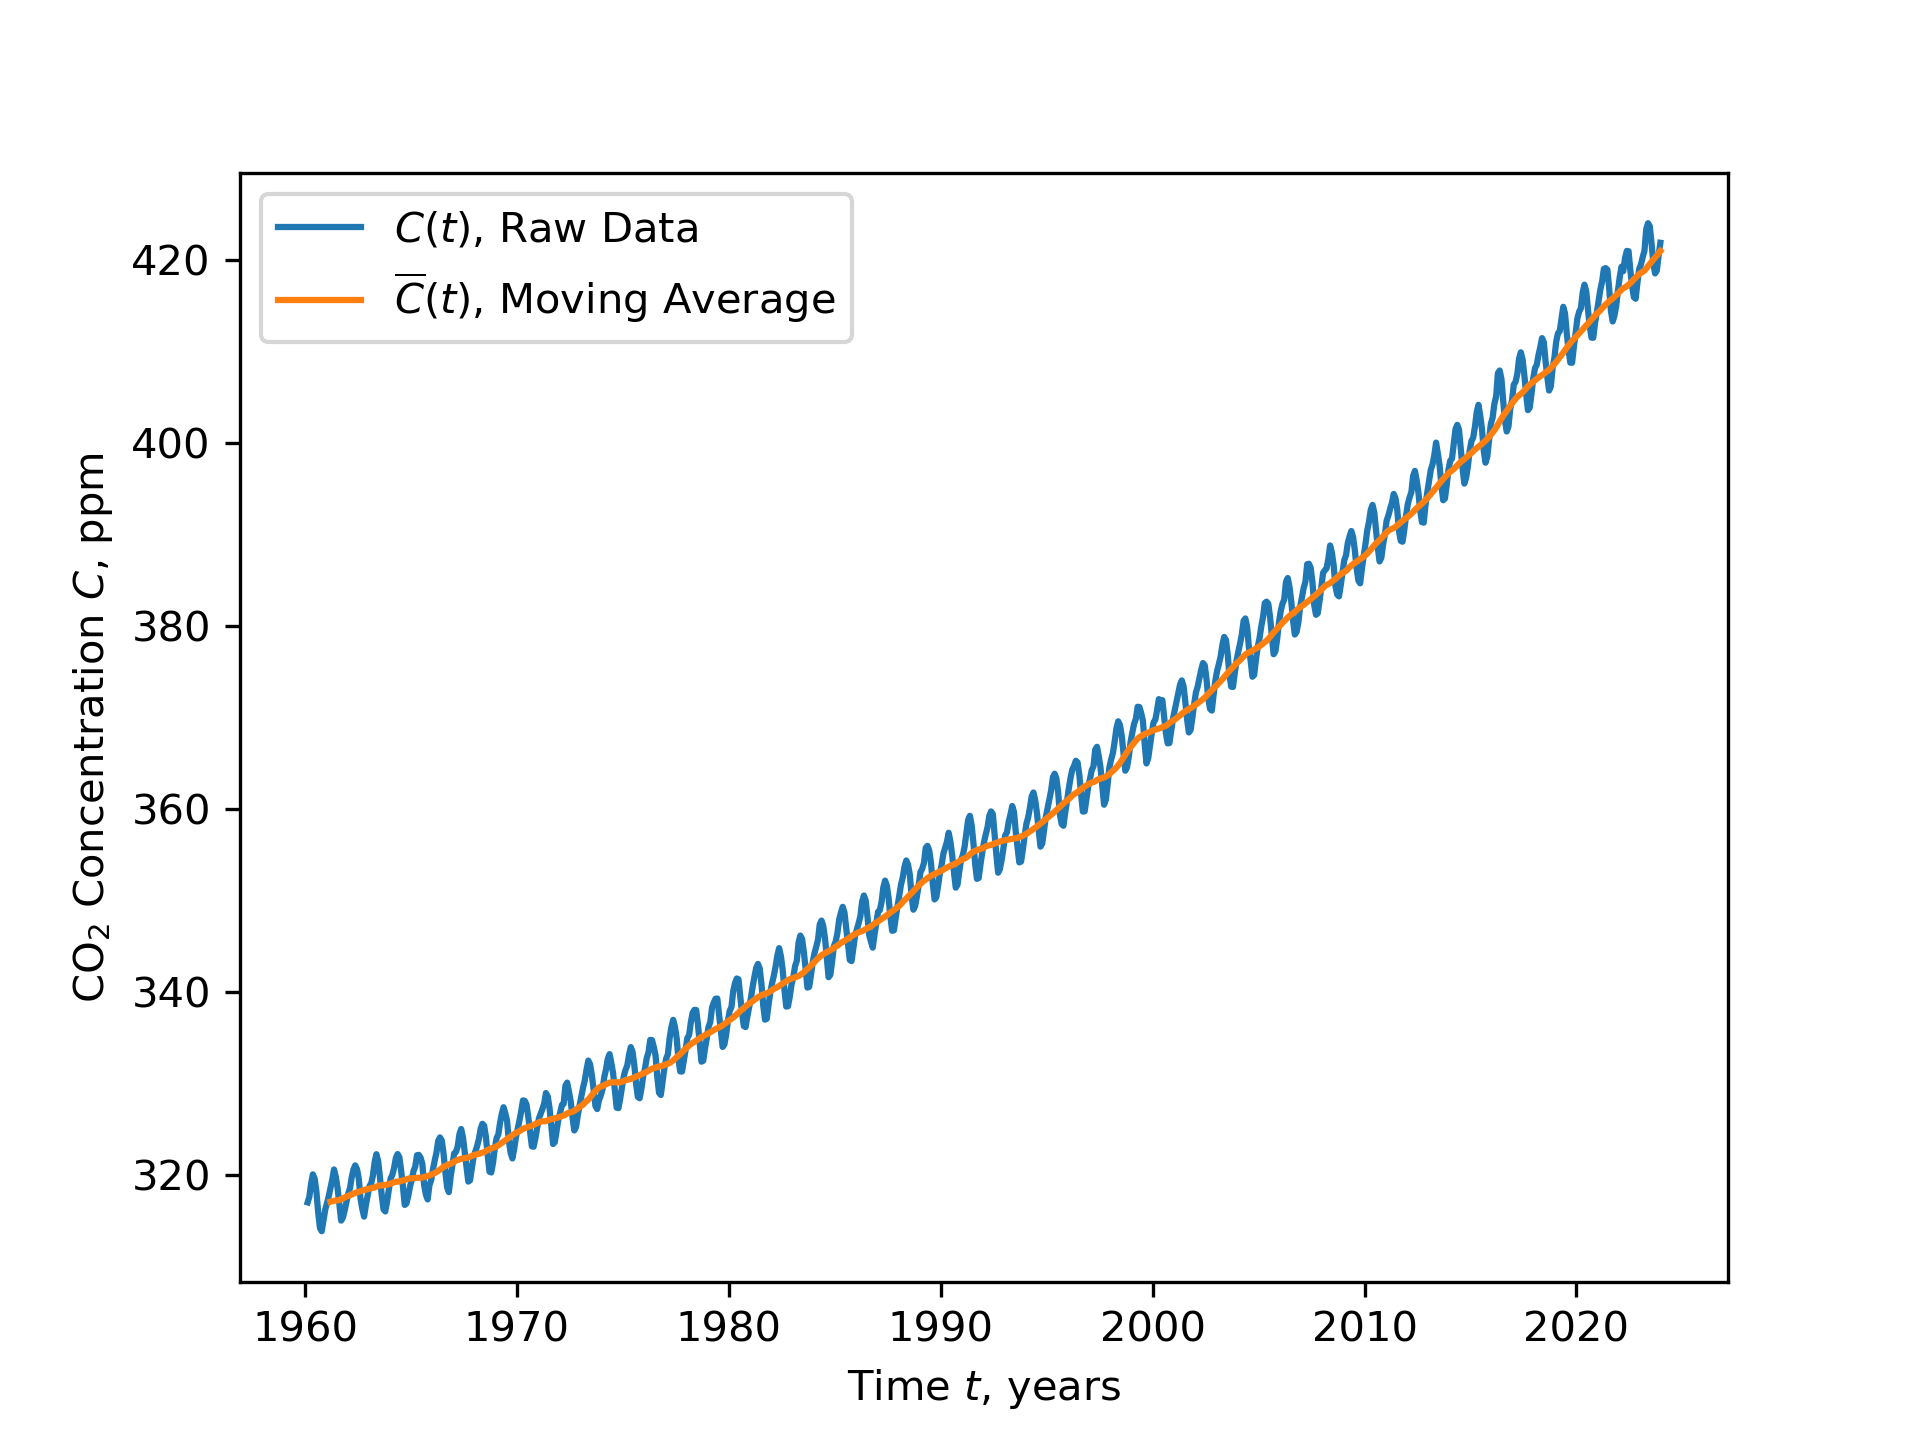
\includegraphics[scale=0.60]{trend0.png}
\]
\end{EnvUplevel}

\begin{EnvUplevel}
The curve $y=\bar C(t)$ looks not quite linear, so we look for a quadratic approximation 
\[
\bar C(t)\approx y(t),
\qquad\text{for}\ y = \a t^2 + \b t + \gamma. 
\]
Standard methods out of scope for this assignment provide the constants
\[
\a = 0.012997,\quad
\b = -50.125,\quad
\gamma = 48631.
\]
\end{EnvUplevel}

\vfill\clearpage

\begin{EnvUplevel}
Here is a plot showing the target curve and approximating parabola defined above:
\[
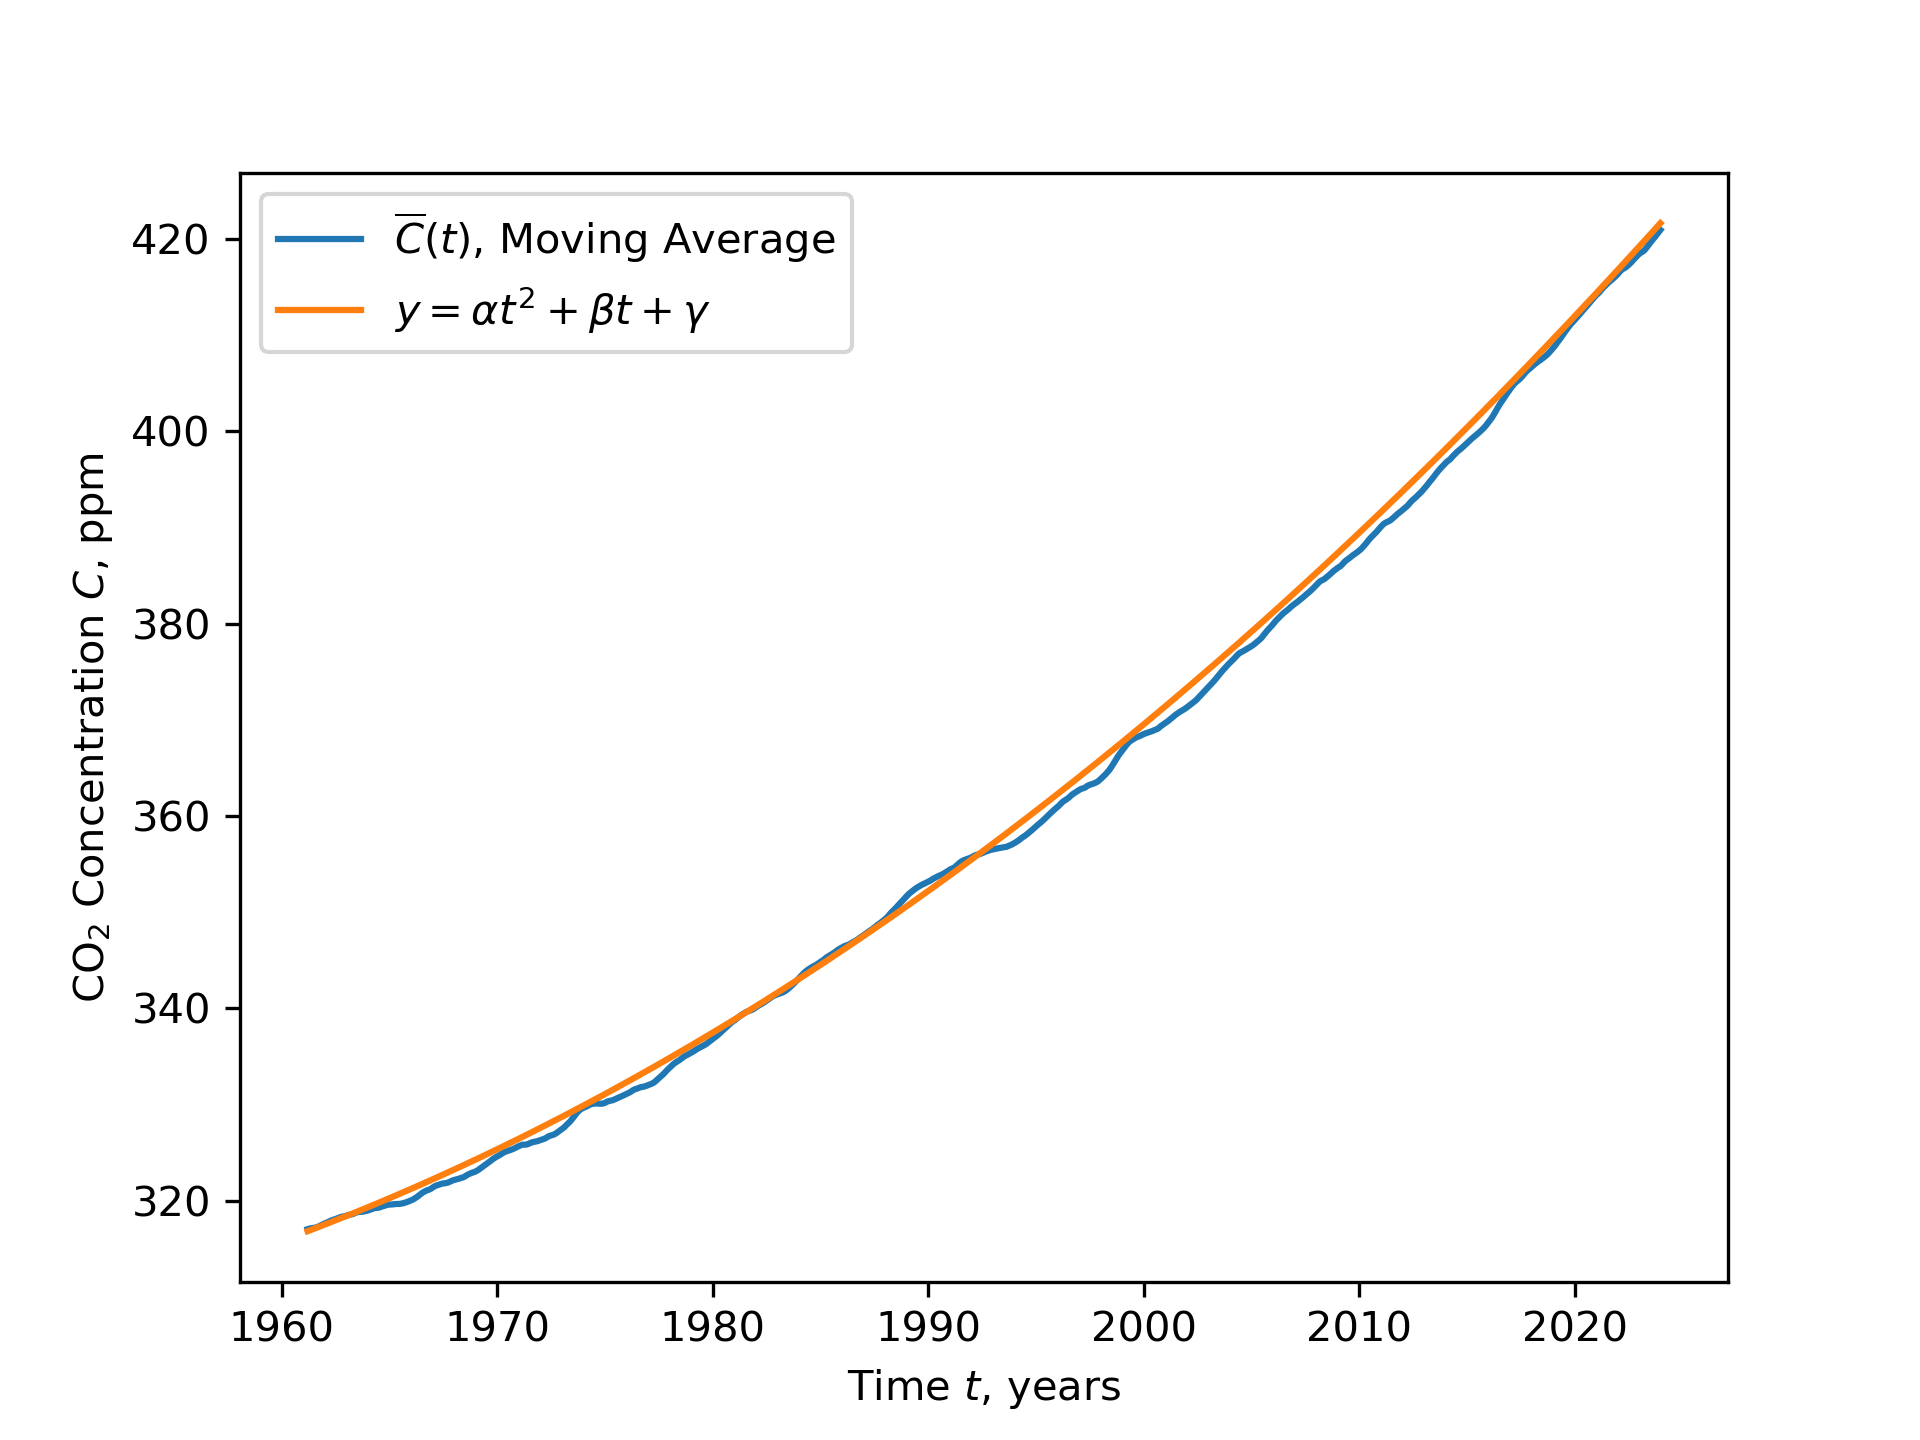
\includegraphics[scale=0.60]{approxy.png}
\] 
\end{EnvUplevel}

\part \twostar \label{co2trend}
Consider an idealized function $C_{101}(t)$ with the form below,
where all the parameters except $t$ are constants:
\[
C_{101}(t) = a t^2 + bt + c + A\cos(2\pi t + \phi).
\]
We want to choose these constants so that the moving average
$\bar C_{101}(t)$ is identical to the approximating parabola
$y=\a t^2 + \b t + \gamma$ plotted above.
Use this criterion to find $a$, $b$, and $c$ to 5-digit accuracy.
\\
({\emph Hint\/}:
Our choice of $r=2\pi/\o=1$ makes the function
$\bar C_{101}(t)$
independent of the cosine term. This is a small extension of
Problem~2(\ref{cosinekiller}): you don't have to prove it.
So, for this part only, it's valid to calculate as if $A=0$
in $C_{101}(t)$.)

\begin{solution}
    After solving the system, we have:
    $$y(t) = \bar{C}_{101}(t) = \frac{1}{3}a+at^{2}-at+bt-\frac{1}{2}b+c$$
    \[ a = 0.012997, b = -50.112003, c = 48605.9396\]
\end{solution}

\begin{EnvUplevel}
Using the values of $a,b,c$ found in part~(\ref{co2trend}) 
and choosing $A=2.8$ and $\phi=0.9\pi$
completes the definition of our approximating function $C_{101}(t)$.
The sketch below shows that the graph of $C_{101}$ tracks the actual measurements
reasonably well.

\[
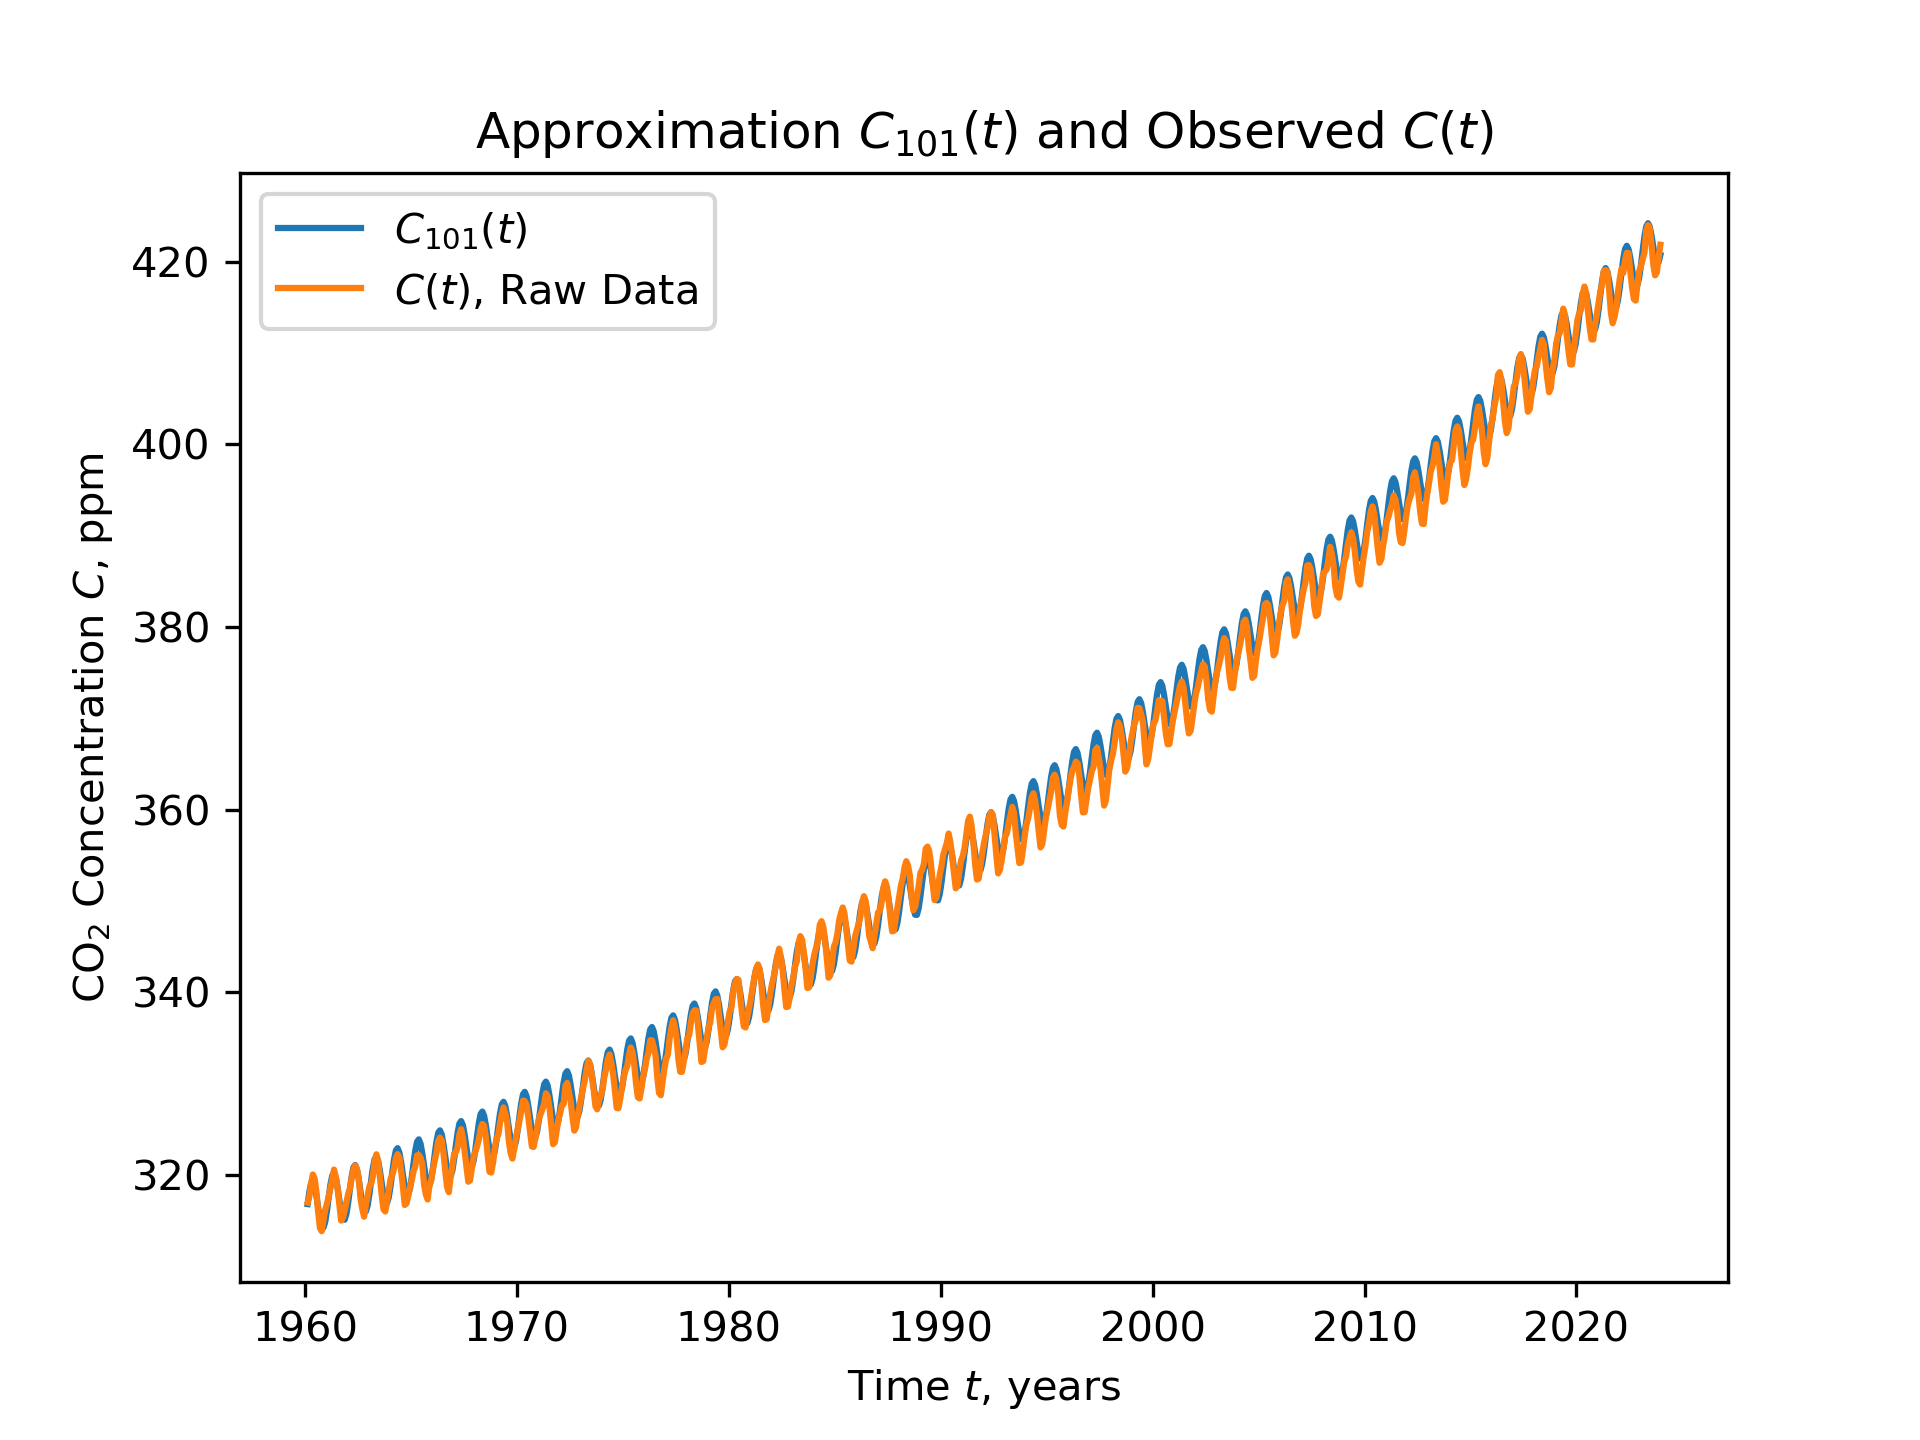
\includegraphics[scale=0.75]{C101andC.png}
\]

\end{EnvUplevel}

\part \onestar
In 2015, the nations of the world met in Paris 
and agreed to limit the average global
temperature to 1.5$^\circ$C above its pre-industrial average.
Then, in 2016, scientists advising the IPCC said that we need
to maintain $C(t)\le 430$ to achieve this goal.
If current trends continue,
in what year will $\bar C_{101}(t)=430$?


\begin{solution}
    Solving our equation from (b) with the definition of $C_{101}$, we get:

    Note that $\frac{1}{2\pi}\sin(2\pi t+0.9\pi)-\frac{1}{2\pi}\sin(2\pi (t-1)+0.9\pi) = 0$, by the periodicity of sine we can just use the quadratic formula.

    \[ 0.012997t^2 - 50.112003t + 48605.9396 + \frac{1}{2\pi}\sin(2\pi t+0.9\pi)-\frac{1}{2\pi}\sin(2\pi (t-1)+0.9\pi) = 430 \]

    Discarding the extraneous solution (i.e., the one that was in the past, which is nonsense), we arrive at.

    \[ t = 2027.474 ~\text{years} \]

    Roughly some time between year 2027 and 2028 then, by this result. In 2027, we will not have reached 430 ppm, and in 2028 we will have surpassed it a little.
\end{solution}




\end{parts}


\end{questions}

\par\vfill\clearpage

\noindent\textbf{Notes and References:}
Statements in the text above are corroborated by
many online sources.
Representative samples are given below.

\begin{itemize}
\item 
The monthly data used to produce the figures here comes from the NOAA,
a government agency in the USA, at this URL:
\url{https://gml.noaa.gov/ccgg/trends/data.html}
\item
The Paris Agreement was announced on 12 December 2015 at the
conclusion of the COP21 climate conference sponsored by the United
Nations. The UN page describing highlights of the agreement is here:
\url{https://unfccc.int/process-and-meetings/the-paris-agreement}
\item
The graph in Fig.~1 is called the Keeling Curve.
The sketch itself comes from the Scripps Institution of Oceanography
at the University of California San Diego, on the ``Full Record'' tab:
see \url{https://keelingcurve.ucsd.edu/}
\item
On the page just cited, the ``2K years'' tab extends the $t$-axis in
Figure~1 back to Year~0 in our current numbering scheme. 
The world's current situation is truly exceptional.
\[
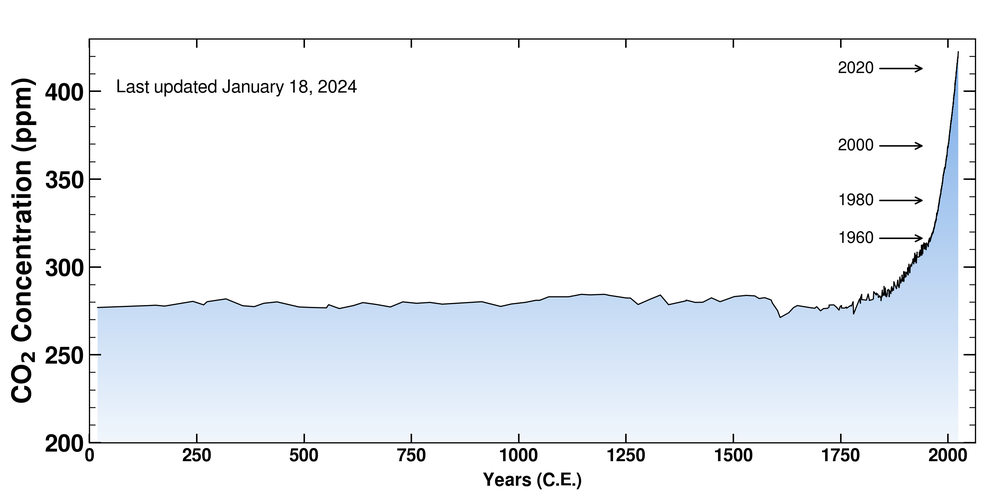
\includegraphics[scale=0.3]{co2_2k_ce.png}
\]
\item
Various credible online sources provide the 430~ppm target for
atmospheric CO$_2$, including \href{https://www.reuters.com/article/idUSKCN1RT0OZ/}{Reuters}:
\begin{quote}
``Science advisers on the Intergovernmental Panel on Climate Change 
have estimated the limits imply an atmospheric CO2 concentration of no more than 
450 parts per million (for 2 degrees) or 430 ppm (for 1.5 degrees).''
\end{quote}
The same group of scientists is cited on the 
\href{https://climate.mit.edu/ask-mit/what-ideal-level-carbon-dioxide-atmosphere-human-life}{MIT Climate Portal}:
\begin{quote}
``In 2016, a worldwide body of climate scientists said that a CO$_2$ level of 430 ppm would push the world past its target for avoiding dangerous climate change.''
\end{quote}
\item
Confronting the facts explored in this assignment can be emotionally difficult.
UBC has gathered some resources to help with this in the online
\href{https://climateemergency.ubc.ca/stem-and-climate-wellbeing-toolkit/}{STEM and Climate Wellbeing Toolkit}.
\end{itemize}
\end{document}
